\section{Motivation}
\begin{frame}{Overview}{}
    \begin{block}{Joint Work -- Its not me alone}
        \centering
        Thorsten Kranz, Gregor Leander, Ko Stoffelen, Friedrich Wiemer
        
\includegraphics[width=0.35\textwidth]{data/logo_rub}
        \hspace{2em}
        
\includegraphics[width=0.45\textwidth]{data/ru_en_branding}
    \end{block}
    \begin{block}{Outline}
        \vspace{0.5em}
%        \begin{itemize}
%            \item Preliminaries
%            \item State of the Art
%            \item Related Work
%            \item Updated State of the Art
%        \end{itemize}
        \tableofcontents
    \end{block}
\end{frame}

\begin{frame}{What is the \textsc{xor} count,}{and why is it important?}
    \begin{block}{Some facts}
    \vspace{-0.5em}
    \begin{itemize}
        \visible<1->{\item Lightweight Block Ciphers}
        \visible<1->{\item Efficient Linear Layers}
        \visible<1->{\item MDS matrices are \enquote{optimal} (regarding security)\footnote{Are they?}}
    \end{itemize}
    \vspace{-0.5em}
    \begin{itemize}
        \visible<2->{\item What is the lightest implementable MDS matrix?}
        \visible<2->{\item What about additional features (Involutory)?}
    \end{itemize}
    \end{block}
    \visible<3->{\begin{block}{The \textsc{xor} count}
    \vspace{-0.5em}
    \begin{itemize}
        \item Metric for needed hardware resources
        \item Smaller is better
    \end{itemize}
    \end{block}}
\end{frame}

\section{Preliminaries}
\begin{frame}{What is an MDS matrix?}{}
%    \begin{columns}
%        \begin{column}{0.45\textwidth}
    \begin{block}{Definition: MDS}
        A matrix $M$ of dimension $k$ over the field $\mathbb{F}$ is \emph{maximum distance separable} (MDS),
        iff all possible submatrices of $M$ are invertible (or nonsingular).
    \end{block}
%        \end{column}
%        \begin{column}{0.45\textwidth}
    \visible<2->{\begin{example}
        The \textsc{Aes MixColumn} matrix is defined over $\mathbb{F}_{2^8} \cong \mathbb{F}[x]/\mathtt{0x11b}$:
        \begin{equation*}
            \begin{pmatrix}
                \mathtt{0x02} & \mathtt{0x03} & \mathtt{0x01} & \mathtt{0x01} \\
                \mathtt{0x01} & \mathtt{0x02} & \mathtt{0x03} & \mathtt{0x01} \\
                \mathtt{0x01} & \mathtt{0x01} & \mathtt{0x02} & \mathtt{0x03} \\
                \mathtt{0x03} & \mathtt{0x01} & \mathtt{0x01} & \mathtt{0x02}
            \end{pmatrix}
            =
            \begin{pmatrix}
                x & x + 1 & 1 & 1 \\
                1 & x & x + 1 & 1 \\
                1 & 1 & x & x + 1 \\
                x + 1 & 1 & 1 & x
            \end{pmatrix}
        \end{equation*}
        This is a (right) \emph{circulant} matrix: $\text{circ}(x, x+1, 1, 1)$.
    \end{example}}
%        \end{column}
%    \end{columns}
\end{frame}
\note{\begin{itemize}
        \item The degree of $\mathbb{F}$ normally fits to the S-box width.
        \item The dimension $k$ resembles the state.
\end{itemize}}

\begin{frame}{What is an MDS matrix?}{Constructions}
    \centering
    \begin{tikzpicture}[%
        mindmap,
        level 1 concept/.append style={%
            level distance=130,
            sibling angle=45,
        },
        scale=0.7, every node/.style={scale=0.7},
    ]

    % Kind of attacks
    \begin{scope}[%
        mindmap,
        concept color=saphierblau,
        text=white,
    ]
        \node [concept] {\textbf{\large MDS}}[clockwise from=45]
        child  {node [concept] (construction) {\textbf{by construction}}[clockwise from=20]
            child {node [concept] (cauchy) {\textbf{Cauchy}}}
            child {node [concept] (vandermonde) {\textbf{Vander\-monde}}}
        }
        child [visible on=<2->] {node [concept] (other) at (2.5, -1) {\textbf{other}}[clockwise from=30]
            child [visible on=<2->] {node [concept] (circ) {\textbf{Circulant}}}
            child [visible on=<2->] {node [concept] (hadamard) {\textbf{Hadamard}}}
            child [visible on=<2->] {node [concept] (toeplitz) {\textbf{Toeplitz}}}
        }
        child [visible on=<3->] {node [concept] (subfield) {\textbf{Subfield}}};
    \end{scope}

    \begin{pgfonlayer}{background}
        \draw (vandermonde)+(2,0) node[scale=0.6] {can be made involutory} ;
        \draw [visible on=<2->] (circ)+(2,0) node[scale=0.6] {used in \textsc{Aes}, \textsc{Gr\o{}stl}, \textsc{Whirlpool}, \textsc{Qarma}, \textsc{Midori}} ;
        \draw [visible on=<2->] (hadamard)+(2,0) node[scale=0.6] {can be made involutory, used in \textsc{Anubis}, \textsc{Khazad}, \textsc{Joltik}} ;
        \draw [visible on=<3->] (subfield)+(2,0) node[scale=0.6] {used in \textsc{Whirlwind}} ;
    \end{pgfonlayer}

    \end{tikzpicture}
\end{frame}

\begin{frame}{What is an MDS matrix?}{Representations}
    \begin{block}{How to implement this in hardware?}
        \begin{itemize}
            \item This is about hardware implementations
            \item How do we implement a \only<1>{field multiplication}\only<2->{\emph{field multiplication}} in hardware?
            \item How do we implement a matrix multiplication in hardware?
        \end{itemize}
    \end{block}
    \visible<2->{%
    \begin{example}
        \begin{columns}
            \begin{column}{0.3\textwidth}
                \centering
        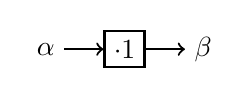
\begin{tikzpicture}
            \node [draw,rectangle,thick,fill=white] (f) {$\cdot 1$};
            \node [left of=f] (x) {$\alpha$};
            \node [right of=f] (y) {$\beta$};
            \draw [->, thick] (x) -- (f);
            \draw [->, thick] (f) -- (y);
        \end{tikzpicture}
            \end{column}
            \begin{column}{0.3\textwidth}
                \centering
        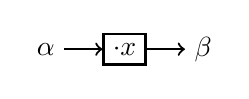
\begin{tikzpicture}
            \node [draw,rectangle,thick,fill=white] (f) {$\cdot x$};
            \node [left of=f] (x) {$\alpha$};
            \node [right of=f] (y) {$\beta$};
            \draw [->, thick] (x) -- (f);
            \draw [->, thick] (f) -- (y);
        \end{tikzpicture}
            \end{column}
            \begin{column}{0.3\textwidth}
                \centering
        \visible<2->{%
        \begin{tikzpicture}
            \node [draw,rectangle,thick,fill=white] (f) {$\cdot (x+1)$};
            \node [left=1em of f] (x) {$\alpha$};
            \node [right=1em of f] (y) {$\beta$};
            \draw [->, thick] (x) -- (f);
            \draw [->, thick] (f) -- (y);
        \end{tikzpicture}}

        \visible<3>{%
        \begin{tikzpicture}
            \node (middle) {\vphantom{.}};
            \node [above=1mm of middle,draw,rectangle,thick,fill=white] (fx) {$\cdot x$};
            \node [below=1mm of middle, draw,rectangle,thick,fill=white] (f1) {$\cdot 1$};
            \node [right=1em of middle, draw,rectangle,thick,fill=white] (xor) {$\oplus$};
            \node [left=2em of middle] (x) {$\alpha$};
            \node [right=1em of xor] (y) {$\beta$};
            \draw [->, thick] (x) -- +(1.5em,0) |- (fx);
            \draw [->, thick] (fx) -| (xor);
            \draw [->, thick] (x) -- +(1.5em,0) |- (f1);
            \draw [->, thick] (f1) -| (xor);
            \draw [->, thick] (xor) -- (y);
        \end{tikzpicture}}
            \end{column}
        \end{columns}
    \end{example}}
\end{frame}

\begin{frame}{Field Multiplication in Hardware}{From $\mathbb{F}_2[x]/p(x)$ to $\mathbb{F}_2^n$}
    \only<1-2>{%
    \begin{block}{Implement \raisebox{-2pt}{\scalebox{0.75}{\tikz{%
            \node[draw,rectangle,thick,fill=black] (f) {$\cdot 1$};
            \node[left of=f] (x) {$\alpha$};
            \node[right of=f] (y) {$\beta$};
            \draw[->, thick] (x) -- (f);
            \draw[->, thick] (f) -- (y);
        }}}}
        \centering
    OK, this one is easy \Winkey{}

    Example in $\mathbb{F}_2[x]/\mathrm{0x13}$:
    \visible<2>{%
        \begin{align*}
            \alpha &= \alpha_0 + \alpha_1 x + \alpha_2 x^2 + \alpha_3 x^3 \\
            %x^4 &\equiv x + 1 \\
            \beta &= \beta_0 + \beta_1 x + \beta_2 x^2 + \beta_3 x^3 \\
                  &= \alpha_0 + \alpha_1 x + \alpha_2 x^2 + \alpha_3 x^3
        \end{align*}
    }
    \end{block}}
    \only<3-4>{%
    \begin{block}{Implement \raisebox{-2pt}{\scalebox{0.75}{\tikz{%
            \node[draw,rectangle,thick,fill=black] (f) {$\cdot x$};
            \node[left of=f] (x) {$\alpha$};
            \node[right of=f] (y) {$\beta$};
            \draw[->, thick] (x) -- (f);
            \draw[->, thick] (f) -- (y);
        }}}}
        \centering
    Example in $\mathbb{F}_2[x]/\mathrm{0x13}$:
    \visible<4>{%
        \begin{align*}
            \alpha &= \alpha_0 + \alpha_1 x + \alpha_2 x^2 + \alpha_3 x^3 \\
            x^4 &\equiv x + 1 \bmod \mathrm{0x13}\\
            \beta &= \beta_0 + \beta_1 x + \beta_2 x^2 + \beta_3 x^3 \\
                  &= x \cdot (\alpha_0 + \alpha_1 x + \alpha_2 x^2 + \alpha_3 x^3) \\
                  &\equiv \alpha_3 + (\alpha_0 + \alpha_3) x + \alpha_1 x^2 + \alpha_2 x^3)
        \end{align*}
    }
    \end{block}}
    \only<5-6>{%
    In matrix notation for $\mathbb{F}_2[x]/\mathrm{0x13}$:
        \begin{align*}
            \beta = 1 \cdot \alpha &\Leftrightarrow \begin{psmallmatrix} \beta_0 \\ \beta_1 \\ \beta_2 \\ \beta_3 \end{psmallmatrix} = \begin{psmallmatrix} 1 & 0 & 0 & 0 \\ 0 & 1 & 0 & 0 \\ 0 & 0 & 1 & 0 \\ 0 & 0 & 0 & 1 \end{psmallmatrix} \cdot \begin{psmallmatrix} \alpha_0 \\ \alpha_1 \\ \alpha_2 \\ \alpha_3 \end{psmallmatrix}\\
            \beta = x \cdot \alpha &\Leftrightarrow \begin{psmallmatrix} \beta_0 \\ \beta_1 \\ \beta_2 \\ \beta_3 \end{psmallmatrix} = \begin{psmallmatrix} 0 & 0 & 0 & 1 \\ 1 & 0 & 0 & 1 \\ 0 & 1 & 0 & 0 \\ 0 & 0 & 1 & 0 \end{psmallmatrix} \cdot \begin{psmallmatrix} \alpha_0 \\ \alpha_1 \\ \alpha_2 \\ \alpha_3 \end{psmallmatrix}
        \end{align*}
    \visible<6>{%
    \begin{block}{Companion Matrix}
        We call $M_{p(x)} = \begin{psmallmatrix} 0 & 0 & 0 & 1 \\ 1 & 0 & 0 & 1 \\ 0 & 1 & 0 & 0 \\ 0 & 0 & 1 & 0 \end{psmallmatrix}$ the \emph{companion matrix} of the polynomial $p(x) = \mathrm{0x13}$.
        For any element $\gamma \in \mathbb{F}_2[x]/p(x)$, we denote by $M_\gamma$ the matrix that implements the multiplication by this element in $\mathbb{F}_2^n$.
    \end{block}}
    }
\end{frame}

\begin{frame}{Counting \textsc{xor}'s}
    \begin{example}
        We can rewrite the \textsc{Aes MixColumn} matrix as:
        \begin{equation*}
            \mathcal{M}_{\mathrm{AES}} = \mathrm{circ}(x, x+1, 1, 1) \cong \mathrm{circ}(M_x, M_{x+1}, M_1, M_1).
        \end{equation*}
        Starting in $\parens{\mathbb{F}_2[x]/\mathrm{0x11b}}^{4 \times 4}$, we end up in $\parens{{\mathbb{F}_2}^{8 \times 8}}^{4 \times 4} \cong {\mathbb{F}_2^{32 \times 32}}$.
    \end{example}
    \visible<2->{%
    \begin{block}{A first \textsc{xor}-count}
        To implement multiplication by $\gamma$, we need $\mathrm{hw}(M_\gamma) - \mathrm{dim}(M_\gamma)$ many \textsc{xor}'s.
        Thus
        \begin{align*}
            \text{\textsc{xor}-count}(\mathcal{M}_{\mathrm{AES}})
                &= 4 \cdot \parens{\mathrm{hw}(M_x) + \mathrm{hw}(M_{x+1}) + 2 \cdot \mathrm{hw}(M_{1})} - 32 \\
                &= 4 \cdot \parens{11 + 19 + 2 \cdot 8} - 32
                 = 152.
        \end{align*}
    \end{block}
    }
\end{frame}

\begin{frame}{The General Linear Group}{Generalise a bit}
    Instead of choosing elements from $\mathbb{F}_{2^n} \cong \mathbb{F}_2[x]/p(x)$ we can extend our possible choices for \enquote{multiplication matrices} by exploiting the following.
    \visible<2->{%
    \begin{alertblock}{Todo}
        Maybe remove this?
    \end{alertblock}}
\end{frame}

\section{State of the Art and Related Work}
\begin{frame}{State of the Art}{Before our Paper}
\end{frame}

\begin{frame}{Related Work I}{}
\end{frame}

\begin{frame}{Related Work II}{}
\end{frame}

\begin{frame}{State of the Art}{After our Paper}
\end{frame}

\section{Future Work}
\begin{frame}{Future Work}{}
\end{frame}
